\documentclass[
ngerman,
twoside,
pdfa=false,
ruledheaders=section,%Ebene bis zu der die Überschriften mit Linien abgetrennt werden, vgl. DEMO-TUDaPub
class=report,% Basisdokumentenklasse. Wählt die Korrespondierende KOMA-Script Klasse
thesis={type=sta},% Dokumententyp Thesis, für Dissertationen siehe die Demo-Datei DEMO-TUDaPhd
accentcolor=TUDa-2c,% Auswahl der Akzentfarbe
custommargins=false,% Ränder werden mithilfe von typearea automatisch berechnet
marginpar=false,% Kopfzeile und Fußzeile erstrecken sich nicht über die Randnotizspalte
%BCOR=5mm,%Bindekorrektur, falls notwendig
parskip=half-,%Absatzkennzeichnung durch Abstand vgl. KOMA-Sript
fontsize=11pt,%Basisschriftgröße laut Corporate Design ist mit 9pt häufig zu klein
%	logofile=tuda_logo.pdf, %Falls die Logo Dateien nicht installiert sind
]{tudapub}

%%%%%%%%%%%%%%%%%%%%%%%%%%%%
% Download des TU-Logos
%%%%%%%%%%%%%%%%%%%%%%%%%%%%
% https://download.hrz.tu-darmstadt.de/protected/CE/TUDa_LaTeX/tuda_logo.pdf
% Der Pfad zum Logo kann als "logofile" angegeben werden.

%%%%%%%%%%%%%%%%%%%
% Sprachanpassung & Verbesserte Trennregeln
%%%%%%%%%%%%%%%%%%%
\usepackage[english, main=ngerman]{babel}
\usepackage[autostyle]{csquotes}% Anführungszeichen vereinfacht
\usepackage{microtype}

%%%%%%%%%%%%%%%%%%%
% Literaturverzeichnis
%%%%%%%%%%%%%%%%%%%
\usepackage{biblatex}   % Literaturverzeichnis
\addbibresource{HausarbeitBib.bib}

%%%%%%%%%%%%%%%%%%%
% Paketvorschläge Tabellen
%%%%%%%%%%%%%%%%%%%
%\usepackage{array}     % Basispaket für Tabellenkonfiguration, wird von den folgenden automatisch geladen
\usepackage{tabularx}   % Tabellen, die sich automatisch der Breite anpassen
%\usepackage{longtable} % Mehrseitige Tabellen
%\usepackage{xltabular} % Mehrseitige Tabellen mit anpassarer Breite
\usepackage{booktabs}   % Verbesserte Möglichkeiten für Tabellenlayout über horizontale Linien

%%%%%%%%%%%%%%%%%%%
% Paketvorschläge Mathematik
%%%%%%%%%%%%%%%%%%%
\usepackage{mathtools} % erweiterte Fassung von amsmath
\usepackage{amssymb}   % erweiterter Zeichensatz
\usepackage[decimalsymbol=comma]{siunitx}   % Einheiten
\usepackage{amsmath}


%%%%%%%%%%%%%%%%%
% Eigenen Pakete Gruppe01
%%%%%%%%%%%%%%%%%%%%
%\usepackage[utf8]{inputenc}
%\usepackage[ngerman]{babel}
\usepackage{hyperref}
\usepackage{graphicx}
\usepackage{subcaption}
\usepackage{listings}
\usepackage[framed, numbered]{matlab-prettifier}
%\usepackage[style=numeric]{biblatex}
%\usepackage{amsthm}
%\usepackage[squaren]{SIunits}
\usepackage{enumitem}
\usepackage{tikz}
\usepackage{pgfplots}
\usepackage{pgfplotstable}
%\usepackage{booktabs}
\pgfplotsset{compat=1.12}
\usepackage{dsfont}

\usepackage{media9}

%%%%%%%%%%%%%%%%%%%
% verschiedene Nummerierung für Abbildungen und Formeln
%%%%%%%%%%%%%%%%%%%
\usepackage{chngcntr}
\counterwithout{equation}{chapter}


%%%%%%%%%%%%%%%%%%%
% Pseudocode
%%%%%%%%%%%%%%%%%%%
\usepackage[linesnumbered,lined,boxruled]{algorithm2e} % Package für Pseudocode

%%%%%%%%%%%%%%%%%%%
% Plotting und Grafik
%%%%%%%%%%%%%%%%%%%
\usepackage{tuda-pgfplots} % Package für Plotting with TUDa mods

%%%%%%%%%%%%%%%%%%%
% Sonstiges
%%%%%%%%%%%%%%%%%%%
\usepackage{blindtext} % Package für Blindtext

\renewcommand{\tt}[1]{\texttt{#1}}

\begin{document}
	
	\title{Ausarbeitung Übung 6}
	%\subtitle{Ein Untertitel, wenn nötig}
	\author[D. Schiller, C. Kramer, S.Arnold, T. Lingenberg]{Dominik Schiller \and Constanze Kramer \and Simon Arnold \and Tobias Lingenberg} %optionales Argument ist die Signatur,
	%\reviewer{Gutachter 1 \and Gutachterin 2} %Gutachten
	
	%Diese Felder werden untereinander auf der Titelseite platziert.
	\department{} % Das Kürzel wird automatisch ersetzt und als Studienfach gewählt, siehe Liste der Kürzel im Dokument.

	
	\date{\today}
	%\examdate{\today}
	
	%	\tuprints{urn=1234,printid=12345}
	%	\dedication{Für alle, die \TeX{} nutzen.}
	
	\maketitle
	\pagenumbering{gobble} % Seitenzahlen angezeigt, startet ab dem Inhaltsverzeichnis
	
	
	%\affidavit
	%\AffidavitSignature
	%\AffidavitSignature
	
	
	%%%%%%%%%%%%%%%%%%%
	%Abstract / Kurzzusammenfassung
	%%%%%%%%%%%%%%%%%%%
	%\include{chapters/zusammenfassung}
	
	%%%%%%%%%%%%%%%%%%%
	%Inhaltsverzeichnis 
	%%%%%%%%%%%%%%%%%%%
	\cleardoublepage
	\tableofcontents % Erstellte ein Inhaltsverzeichnis
	
	%\cleardoublepage
	\pagenumbering{arabic} % Seitenzahlen angezeigt, startet ab dem Inhaltsverzeichnis
	\setcounter{page}{1} % Setzt den Seitenzahlenzähler auf 1
	
	%%%%%%%%%%%%%%%%%%%%%%%%%%%%%%%%%%%%%%%%%%%%%%%%%%%%%%%%%%%%%%%%%%%%%%%%%%%%%%%%%%%%%%%%%%%%%%%%%%
	
	% INHALT, am Besten ausgelagert in eigene Files/Kapitel und dann mit \include{Unterordner/Filename} eingefügt, sorgt für bessere Übersichtlichkeit und Fehlersuche. Einzelne Dateien sind aktuell im Ordner Sections abgelegt. 
	%%%%%%%%%%%%%%%%%%Einleitung%%%%%%%%%%%%%%%%%
	\chapter{Einleitung}\label{sec:intro}
Diese Arbeit beschäftigt sich mit dem Übungsblatt 7 des Faches \glqq Einführung in die numerische Berechnung elektromagnetischer Felder\grqq{}. Zunächst wird die skalare Laplace-Gleichung für den 2D-Fall hergeleitet. Anschließend wird durch Einsetzen der Maxwell- und Materialgleichungen die gedämpfte Wellengleichung hergeleitet.
Es wird ein Kondensator mit linear-variierender Permittivität mit Hilfe der Methode der Finiten Integration simuliert und das Ergebnis in ParaView analysiert. 
Abschließend wird ein Beschleunigermagnet in FEMM simuliert und die Stärke der Homogenität sowie die Sättigung der Eisenteile überprüft. 
	%%%%%%%%%%%%%%%%%%Haupteil%%%%%%%%%%%%%%%%%%%
	\chapter{Bearbeitung der Übungsaufgaben}
\section{Stetigkeitsbedingung des Stromes}
Mithilfe des Ampereschen Gesetzes

\begin{equation}
\label{gl:ampere}
\operatorname{rot} \vec{H}(\vec{r},t) = \frac{\partial\vec{D}(\vec{r},t)}{\partial t}
+ \vec{J}(\vec{r},t)
\end{equation} 

und des Gaussschen Gesetzes

\begin{equation}
\label{gl:gauss}
\operatorname{div} \vec{D}(\vec{r},t) = \varrho (\vec{r},t),
\end{equation}

lässt sich die Kontinuitätsgleichung (siehe Gleichung \ref{gl:kontinu}) herleiten.
Bildet man auf beiden Seiten der Gleichung \ref{gl:ampere} die Divergenz der Vektorfelder erhält man

\begin{equation*}
\operatorname{div} \operatorname{rot} \vec{H}(\vec{r},t) = \operatorname{div} \left( \frac{\partial\vec{D}(\vec{r},t)}{\partial t} + \vec{J}(\vec{r},t) \right),
\end{equation*} 

wobei $\operatorname{div} \operatorname{rot} \vec{a} = 0$ und $\operatorname{div} (\vec{a}+\vec{b}) = \operatorname{div} \vec{a} + \operatorname{div} \vec{a}$ gilt. Es ergibt sich die Gleichung

\begin{equation*}
\frac{\partial}{\partial t}\operatorname{div}\vec{D}(\vec{r},t) + \operatorname{div}\vec{J}(\vec{r},t) = 0.
\end{equation*}

Setzt man zuletzt nun Gleichung \ref{gl:gauss} ein erhält man die Kontinuitätsgleichung

\begin{equation}
\label{gl:kontinu}
\frac{\partial \varrho (\vec{r},t)}{\partial t} + \operatorname{div}\vec{J}(\vec{r},t) = 0.
\end{equation}

Aus Gleichung \ref{gl:kontinu} soll nun die Stetigkeitsbedingung für die Stromdichte bestimmt werden. Hierzu werden Überlegungen an einer Grenzfläche unternommen. Gleichung \ref{gl:kontinu} wird auf beiden Seiten über ein quaderförmiges  Volumen $V$ integriert, durch das die Grenzfläche verläuft (siehe Abbildung \ref{fig:grenz}).

\begin{figure}[thbp]
	\centering
	\includegraphics[width=.5\textwidth]{data/Grenzfläche}
	\caption{Grenzfläche zwischen zwei Vektorfeldern $\vec{J_1}$ und $\vec{J_1}$ mit eingeführtem Quadervolumen $V$}
	\label{fig:grenz}
\end{figure}

Durch dieses Vorgehen erhält man die Gleichung

\begin{equation*}
\int\limits_{V}^{} \operatorname{div}\vec{J}(\vec{r},t) \ dV = -\frac{\partial}{\partial t} \int\limits_{V}^{} \varrho (\vec{r},t) \ dV.
\end{equation*}

Mithilfe des Integralsatz von Gauss (siehe Gleichung \ref{gl:integralsatz})
\begin{equation}
\label{gl:integralsatz}
\int\limits_{V}^{} \operatorname{div}\vec{F} \ dV = \int\limits_{\partial V}^{} \vec{F} \ d\vec{A}
\end{equation}
Ergibt sich der erste Teil der Gleichung zu 
\begin{equation*}
\int\limits_{\partial V}^{} \vec{J}(\vec{r},t) \ d\vec{A} = -\frac{\partial}{\partial t} \int\limits_{V}^{} \varrho (\vec{r},t) \ dV.
\end{equation*}
Hierbei beschreibt $\partial V$ den Rand des Volumens. Es handelt sich nun um ein Oberflächenintegral, die Dimension wurde um eins verringert.

Das Volumenintegral über die Raumladungsdichte $\varrho$ im zweiten Teil der Gleichung lässt sich durch die Gesamtladung $Q_V$ innerhalb des gedachten Volumens $V$ ersetzen.
\begin{equation*}
\int\limits_{\partial V}^{} \vec{J}(\vec{r},t) \ d\vec{A} = -\frac{\partial Q_V(t)}{\partial t}.
\end{equation*}

Die Seitenflächen des Quaders, die senkrecht zu der Grenzfläche liegen, werden nun als vernachlässigbar klein angenommen. Demnach müssen für das Oberflächenintegral nur noch die zwei Stirnflächen $A$ mit Normalenvektor $\vec{n}_1$ und $\vec{n}_2$ betrachtet werden, die fast auf der Grenzfläche liegen. Oberhalb der Grenzfläche liegt das Vektorfeld $\vec{J_1}$, unterhalb $\vec{J_2}$ vor. Da die Normalenvektoren in unterschiedliche Richtung zeigen ergibt sich die Gleichung
\begin{equation*}
\int\limits_{A}^{} \vec{J_1}(\vec{r},t) \ d\vec{A} - \int\limits_{A}^{} \vec{J_2}(\vec{r},t) \ d\vec{A} = -\frac{\partial Q_A(t)}{\partial t}.
\end{equation*}
Ist Fläche $A$ nun selbst infinitesimal klein, so kann $\vec{J_1}$ und $\vec{J_2}$ auf der gesamten Fläche als konstant angenommen werden. Die Integrale lassen sich zu 
\begin{equation*}
A(\vec{J_1}-\vec{J_2})\cdot \vec{n}
\end{equation*}
vereinfachen. Auch die Flächenladung $Q_A$ kann bei einer unendlich kleinen Fläche wieder durch die Flächenladungsdichte $\varrho_A$ beschreiben werden  mit $Q_A =\varrho_A \cdot A $. Abschließend ergibt sich

\begin{equation*}
A(\vec{J_1}(t)-\vec{J_2}(t))\cdot \vec{n} = \frac{\partial \varrho_A(t) \cdot A}{\partial t}
\end{equation*}
und nach kürzen von $A$
\begin{equation}
\label{gl:stetig}
(\vec{J_1}(t)-\vec{J_2}(t))\cdot \vec{n} = \frac{\partial \varrho_A(t)}{\partial t}
\end{equation}

Formel \ref{gl:stetig} trifft nun Aussagen über die Stetigkeit der Stromdichte $\vec{J}$ an einer Grenzfläche. $\vec{J_1}$ und $\vec{J_2}$ sind stetig in normaler Richtung, wenn $\frac{\partial \varrho_A}{\partial t} = 0$ gilt, also sich die Ladungsdichte an der Grenzfläche nicht zeitlich verändert.
	
\section{Überspannungsableiter}
Im Folgenden wird mit Hilfe des Simulationsprogramms FEMM das Modell eines Überspannungsableiters erstellt und das tangentiale Elektrische Feld $E_t$ entlang der Mittelachse des Ableiters unter verschiedenen Bedingungen ermittelt. \\ \\
Um das Modell zu erzeugen wurde eine OctaveFEMM Routine geschrieben, diese ist unter dem Namen \tt{Aufgabe6\_2a.m} im Anhang zu finden. Als Parameter nimmt sie den Außendurchmesser \tt{d} des Rings entgegen und dessen Höhe \tt{z}. Der Parameter \tt{meshnet} bestimmt die Größe der zum Meshen benutzen Dreiecke. Es ist zu erwähnen, dass Kanten des unteren Mast und Teile der Antenne nicht modelliert werden, da sie beim Meshen nicht berücksichtigt werden sollen. Setz man dort die Materialproperty \tt{<No Mesh>}, um zu verhindern, dass diese gemesht werden, so endet das Programm mit einer Fehlermeldung.\\ \\
In Abbildung \ref{fig:Alle} ist der Überspannungsableiter sowie das entstehende Potenzial im Raum zu sehen. Die Randbedingungen werden für die rechte und die obere Begrenzung des Spannungsableiters gesetzt. Abb. \ref{fig:KeinRand} zeigt die Entwicklung des Potenzial, wenn keine Randbedingungen gesetzt wurden. Abb. \ref{fig:0VRand} hingegen zeigt das Potenzial, wenn am Rand die Bedingung von \SI{0}{\volt} gesetzt wird. Am oberen Mast, sowie an allen damit verbundenen leitenden PEC-Gebieten und am feldsteuernden Ring liegt ein Potenzial von \SI{471000}{\volt} an. Am Boden und am unteren Mast liegt das Potenzial \SI{0}{\volt} an. \\ \\
Da der Überspannungsableiter in der Realität nicht in einem geerdeten Kasten steht, ist es sinnvoller die Berechnung ohne explizite Randbedingungen durchzuführen. 
\newpage
\begin{figure}[h!]
	\centering
	\begin{subfigure}[h]{.28\textwidth}
		\centering
		\includegraphics[width=\textwidth]{data/Skala}
		\caption{Skala}
		\label{fig:Skala}
	\end{subfigure}
	\begin{subfigure}[h]{.35\textwidth}
		\centering
		\includegraphics[width=\textwidth]{data/NoBoundary}
		\caption{Entwicklung des Potenzials ohne explizite Randbedingung}
		\label{fig:KeinRand}
		\vspace{-2pt}
	\end{subfigure}
	\begin{subfigure}[h]{.34\textwidth}
		\centering
		\includegraphics[width=\textwidth]{data/0VBoundary}
		\caption{Entwicklung des Potenzials mit Randbedingung \SI{0}{\volt}}
		\label{fig:0VRand}
	\end{subfigure}
	\caption{Überspannungsableiter mit unterschiedlichen Randbedingungen}
	\label{fig:Alle}
\end{figure}
\newpage
Darüber hinaus wurde untersucht, wie sich das tangentiale Elektrische Feld entlang der Symmetrieachse entwickelt. Das Feld wurde nur in den Ableitersegmenten in der Höhe zwischen \SI{2000}{\milli\meter} und \SI{5480}{\milli\meter} berechnet. In Abbildung \ref{fig:Vgl} sind die Stärken der tangentialen Elektrischen Felder zu sehen. Der blaue Graph entsteht, wenn keine Randbedingungen vorgegeben werden, der rote bei der Randbedingung \SI{0}{\volt}. Es ist zu erkennen, dass das elektrische Feld bei der Randbedingung \SI{0}{\volt} mit zunehmender Höhe deutlich stärker wird, als das Feld ohne Randbedingungen. \\ \\

\begin{figure}[h]
	\centering
	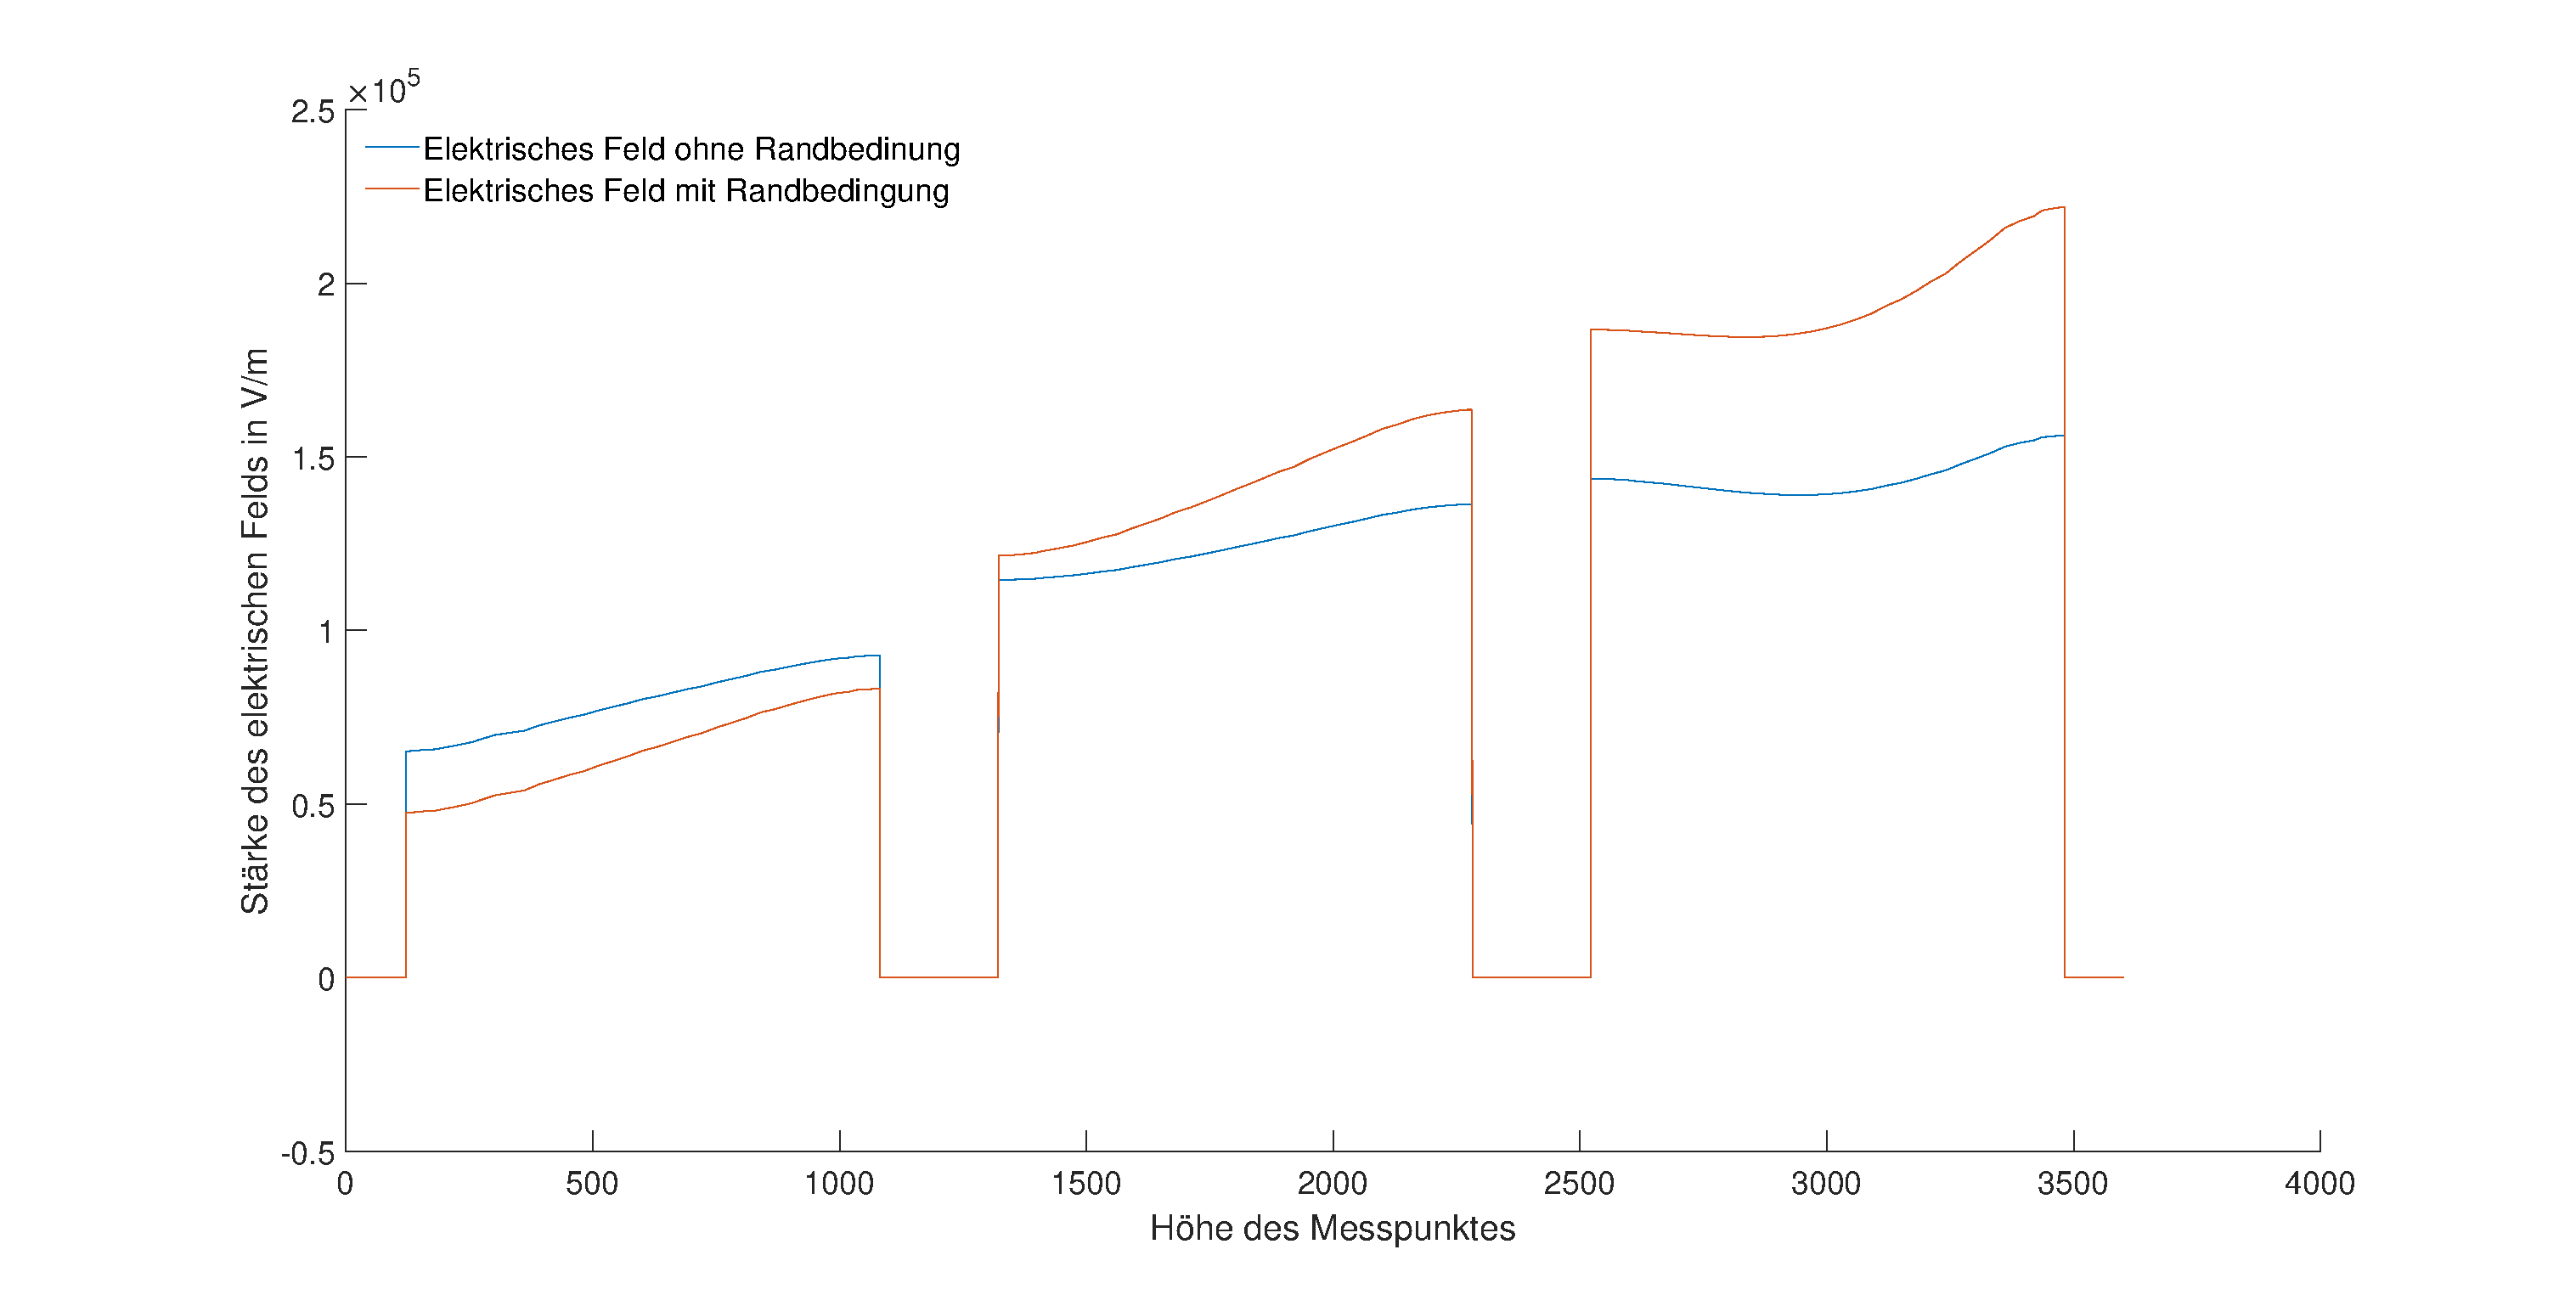
\includegraphics[width=\textwidth]{data/VergleichRandbedingung}
	\caption{Vergleich des tangentialen elektrischen Feldes bei unterschiedlichen Randbedingungen}
	\label{fig:Vgl}
\end{figure}


Zusätzlich gibt es bei FEMM die Möglichkeit das Gitter, das zum Meshen benutzt wird manuell einzustellen bzw. zu beeinflussen. Der Routine \tt{Aufgabe6\_2} wurden 120 unterschiedliche Netzgrößen von 10, bis minimal 0.8 übergeben und anschließend das tangentiale elektrische Feld berechnet. In Abbildung \ref{fig:Netz} sind diese Felder zu sehen. Bei der Verfeinerung des Gitters ließ sich kein Wert ermitteln, ab dem sich das Feld nicht mehr verändert. Beobachtet werden konnte, dass die maximale Netzgröße mit der FEMM arbeitet 10 und die minimale 0.8 beträgt. Der zum Vergleichen gewählte Messpunkt hat die Höhe \SI{4600}{\milli\meter}, auffällig ist, dass ab einer Netzgröße kleiner als eins (Messpunkt 100) die Rechenergebnis sehr stark variieren, wie in Abb. \ref{fig:NetzVGL} deutlich wird. \\ \\

\begin{figure}
	\centering
	\begin{subfigure}[h]{.8\textwidth}
		\centering
		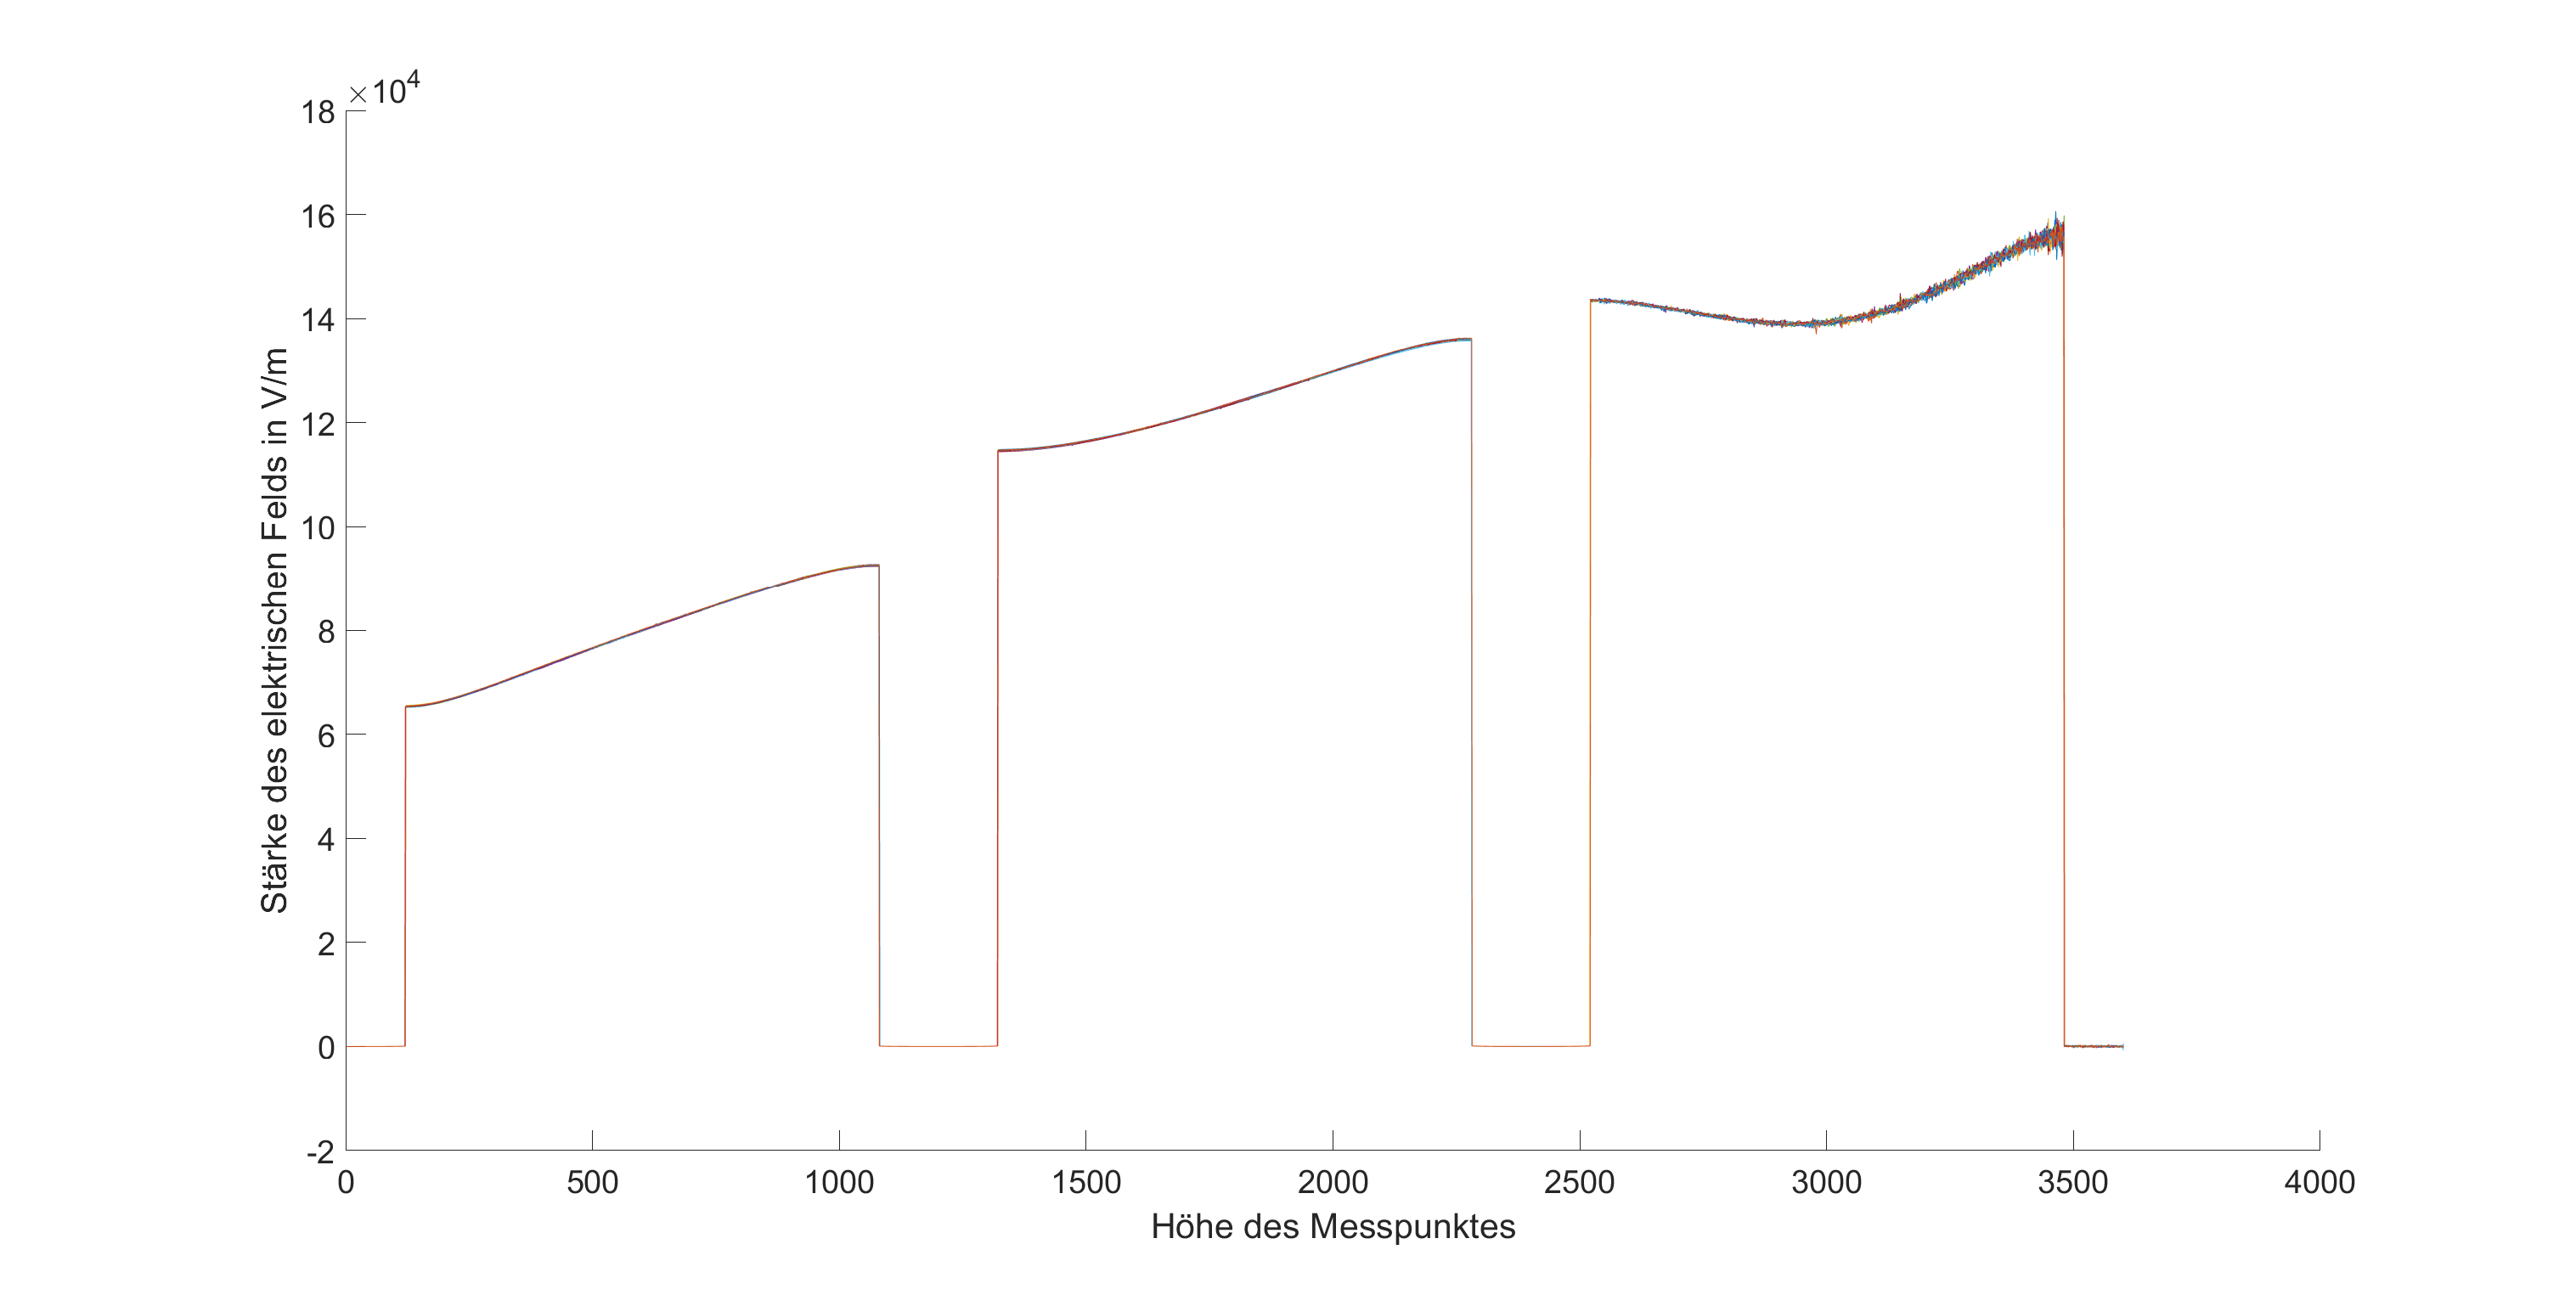
\includegraphics[width=\textwidth]{data/NetzVefeinerung}
		\vspace*{-28pt}
		\caption{Das tangentiale elektrische Feld mit unterschiedlichen Netzgrößen}
		\label{fig:Netz}
		
	\end{subfigure}
	
	\begin{subfigure}[h]{.8\textwidth}
		\centering
		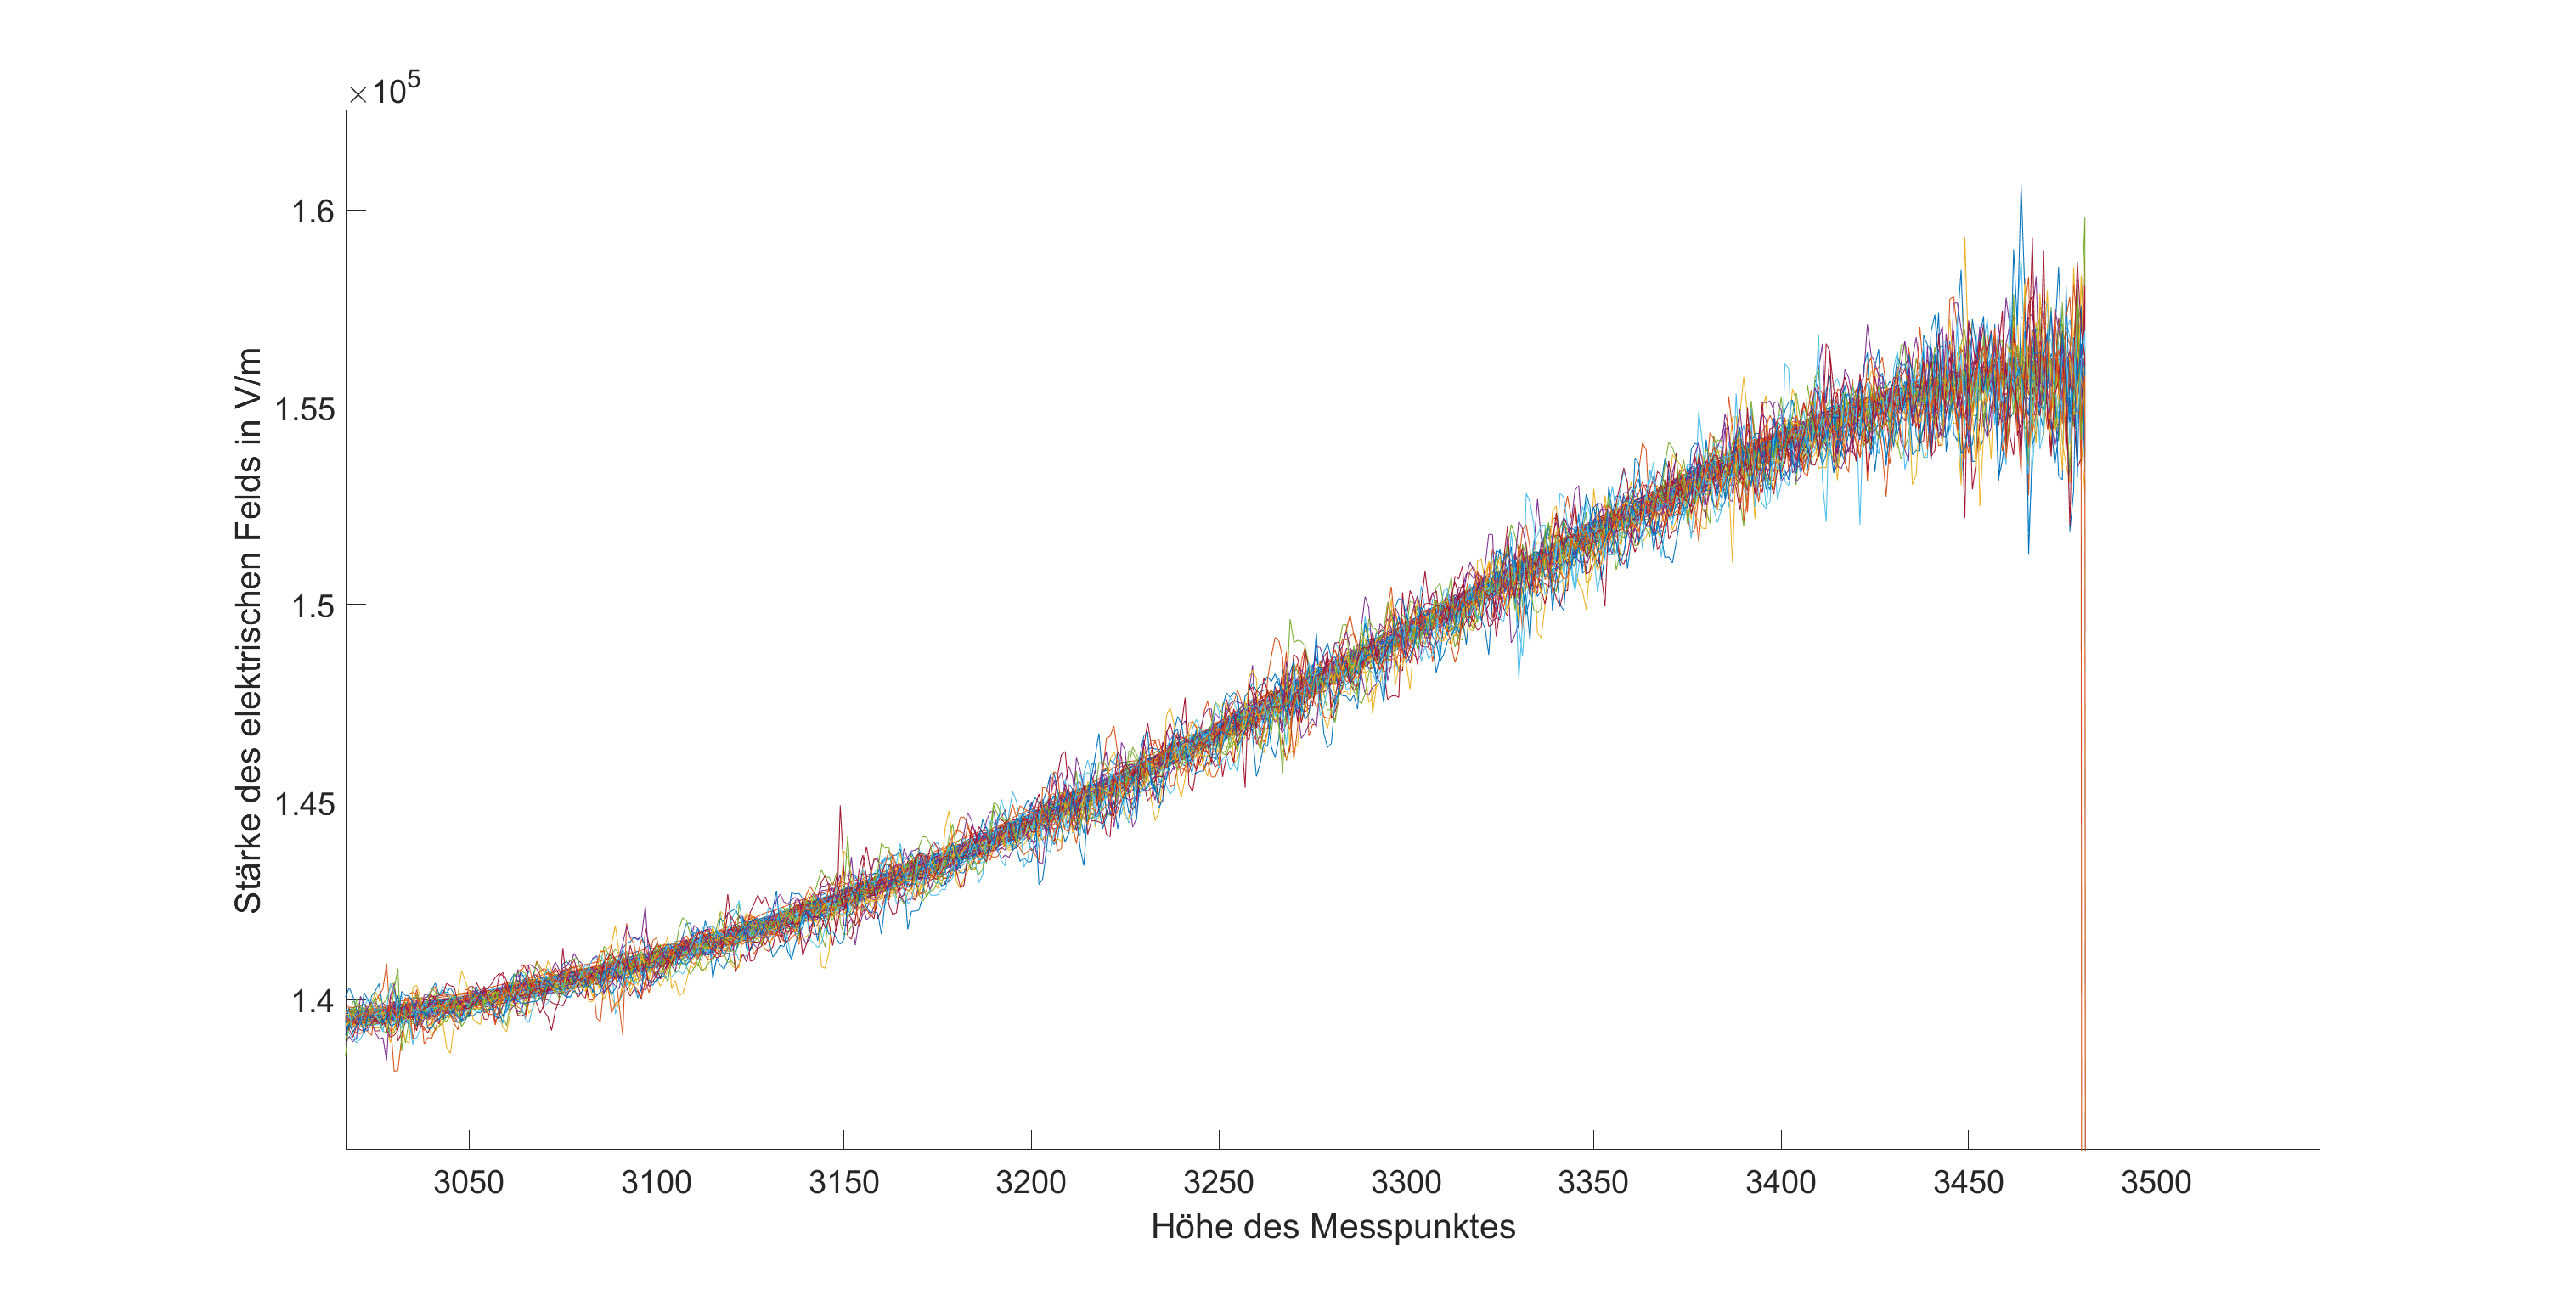
\includegraphics[width=\textwidth]{data/NetzVefeinerungGroß}
		\caption{Detailausschnitt von \ref{fig:Netz}}
		\label{fig:NetzGroß}
	\end{subfigure}
	
	\begin{subfigure}[h]{.8\textwidth}
		\centering
		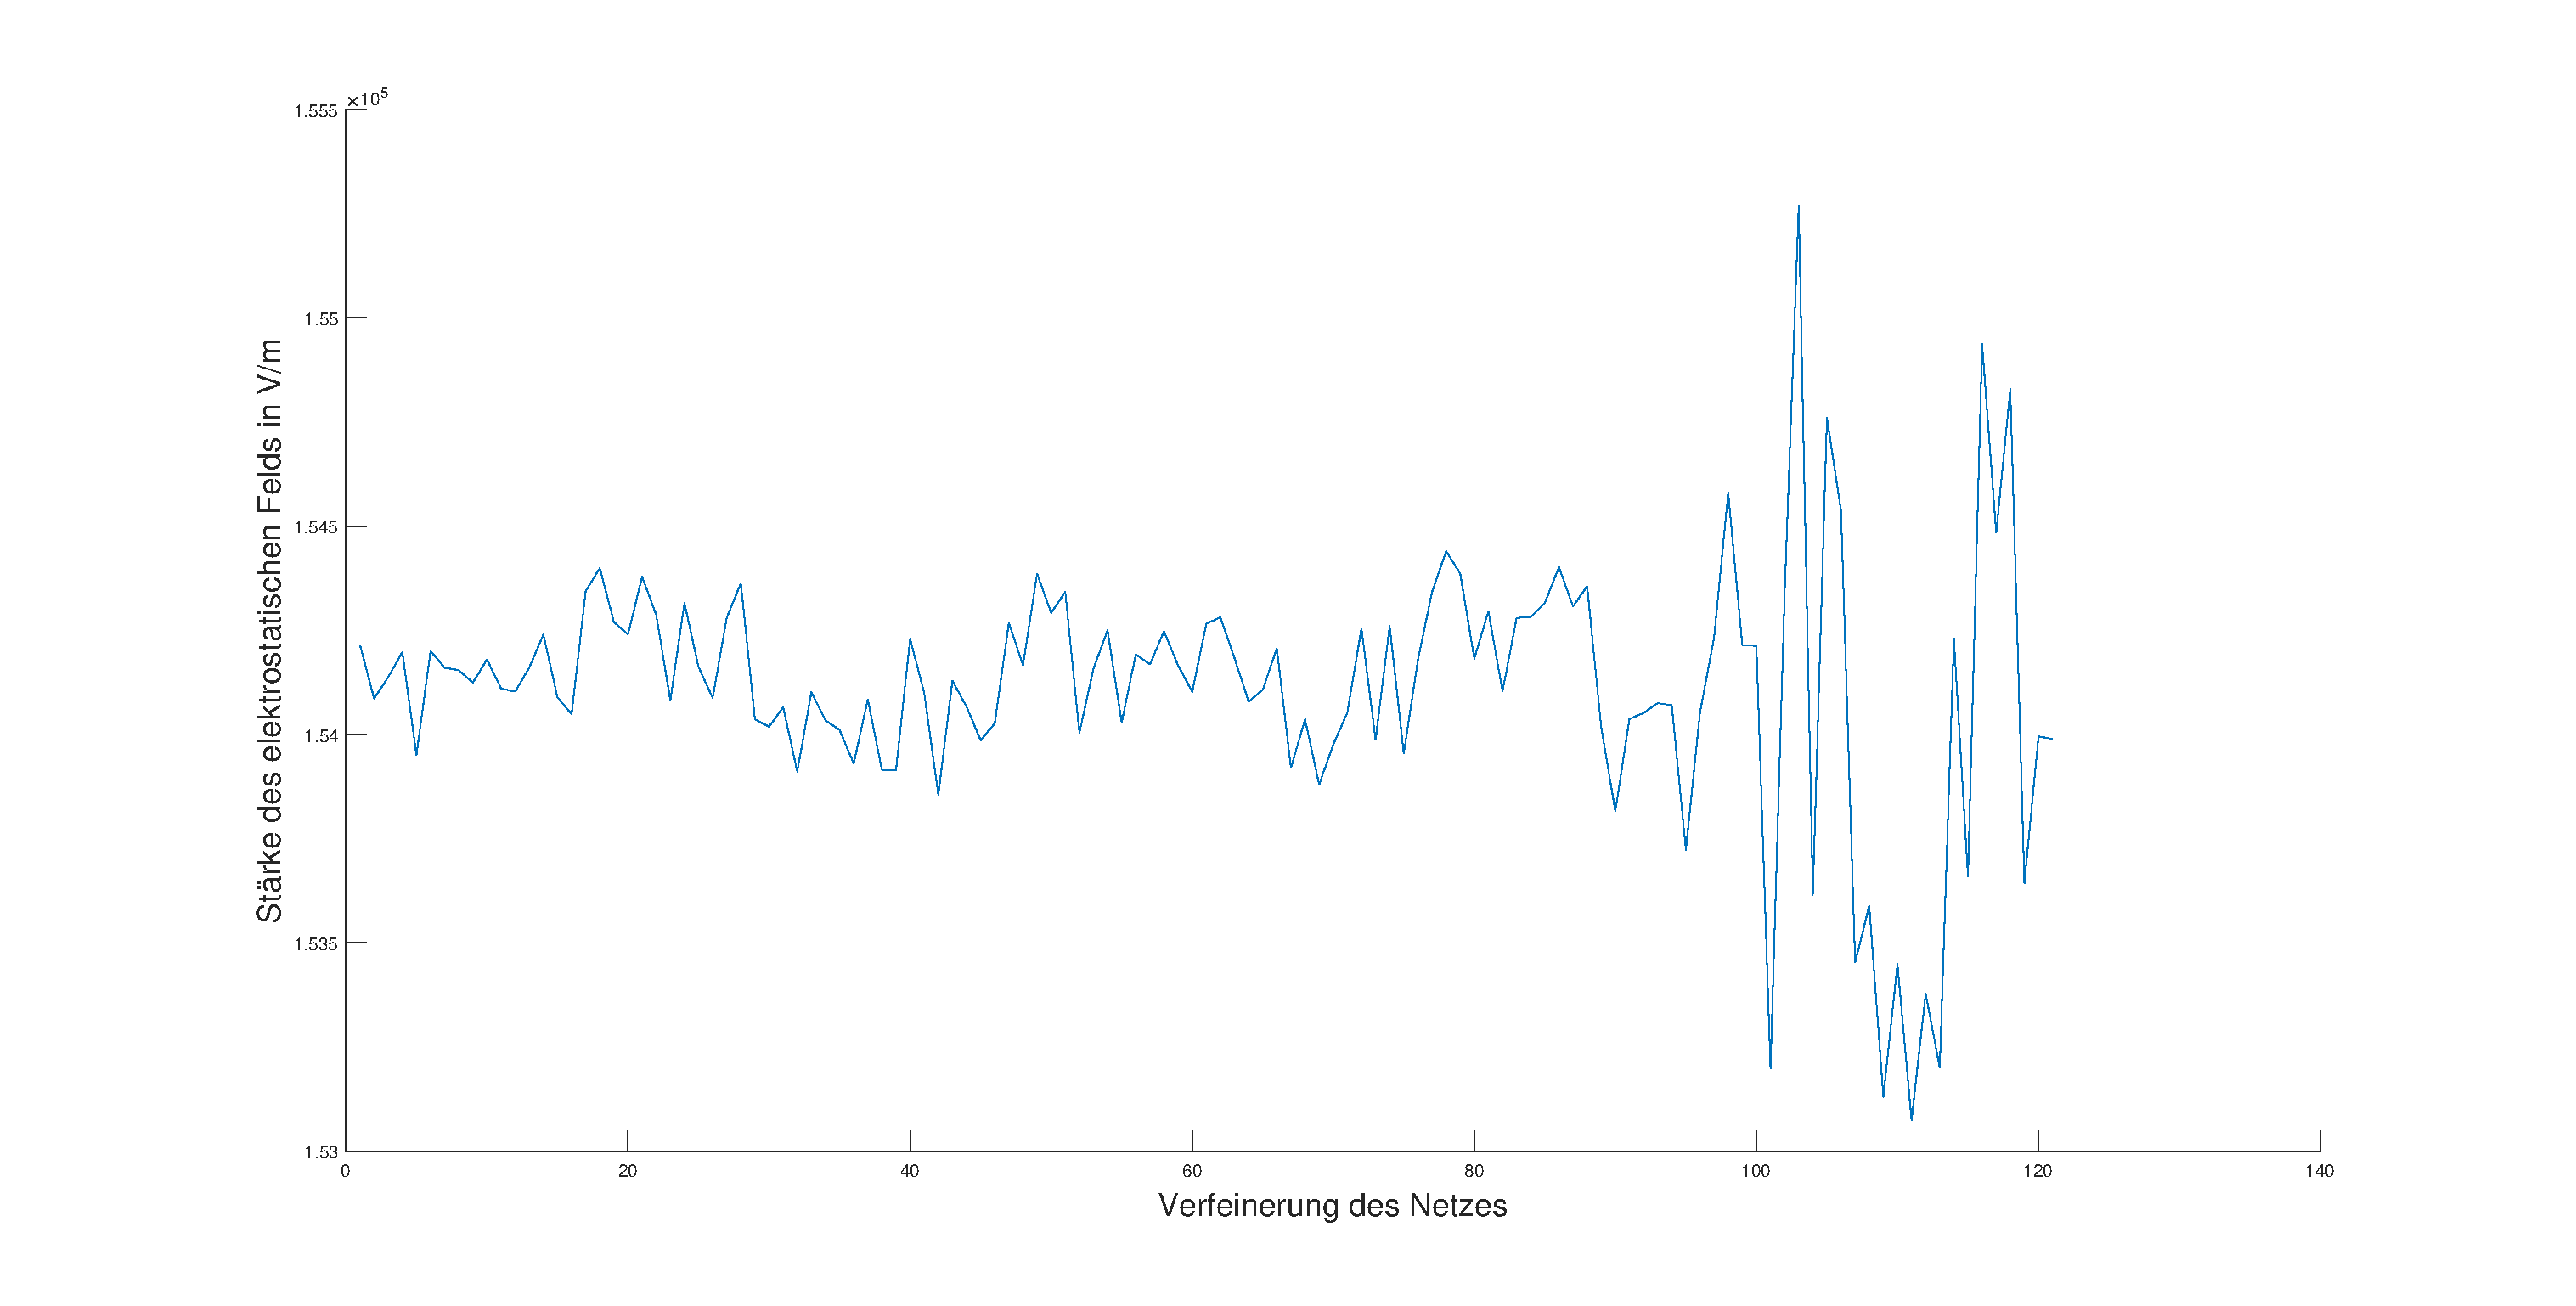
\includegraphics[width=\textwidth]{data/NetzVergleich}
		\caption{Stärke des elektrischen Feldes, abhängig von der gewählten Netzgröße}
		\label{fig:NetzVGL}
	\end{subfigure}
	\caption{Auswirkung der Verfeinerung des Gitters, das FEMM zum Meshen benutzt}
	
	%\label{fig:Alle}
\end{figure}

\newpage

Des Weiteren wurde die Auswirkung des feldsteuernden Rings auf das tangentiale elektrische Feld betrachtet. Zur Visualisierung des elektrischen Felds wurde der Octave Befehl \tt{surf} benutzt. Dadurch ist es möglich einen dreidimensionalen Plot zu erzeugen. Das elektrische Feld hängt dabei von der Höhe des Messpunktes und dem Außendurchmesser $d_a$ des Rings ab, dieser variiert zwischen \SI{600}{} und \SI{2000}{\milli\meter}. Dem  Modell wurden keine Randbedingungen vorgegeben. \\
Die tangentialen elektrischen Felder sind in der Abbildung \ref{fig:3DTang} zu sehen. Auffällig ist, dass bei steigendem Abstand zwischen dem Ring und dem Mast sich die elektrischen Felder unterschiedlich verändern. Das elektrische Feld in dem oberen und mittleren Ableitersegment nimmt ab, während es im untersten Segment ein stärkeres Feld entsteht.
\begin{figure}[h]
	\begin{subfigure}[h]{\textwidth}
		\centering
		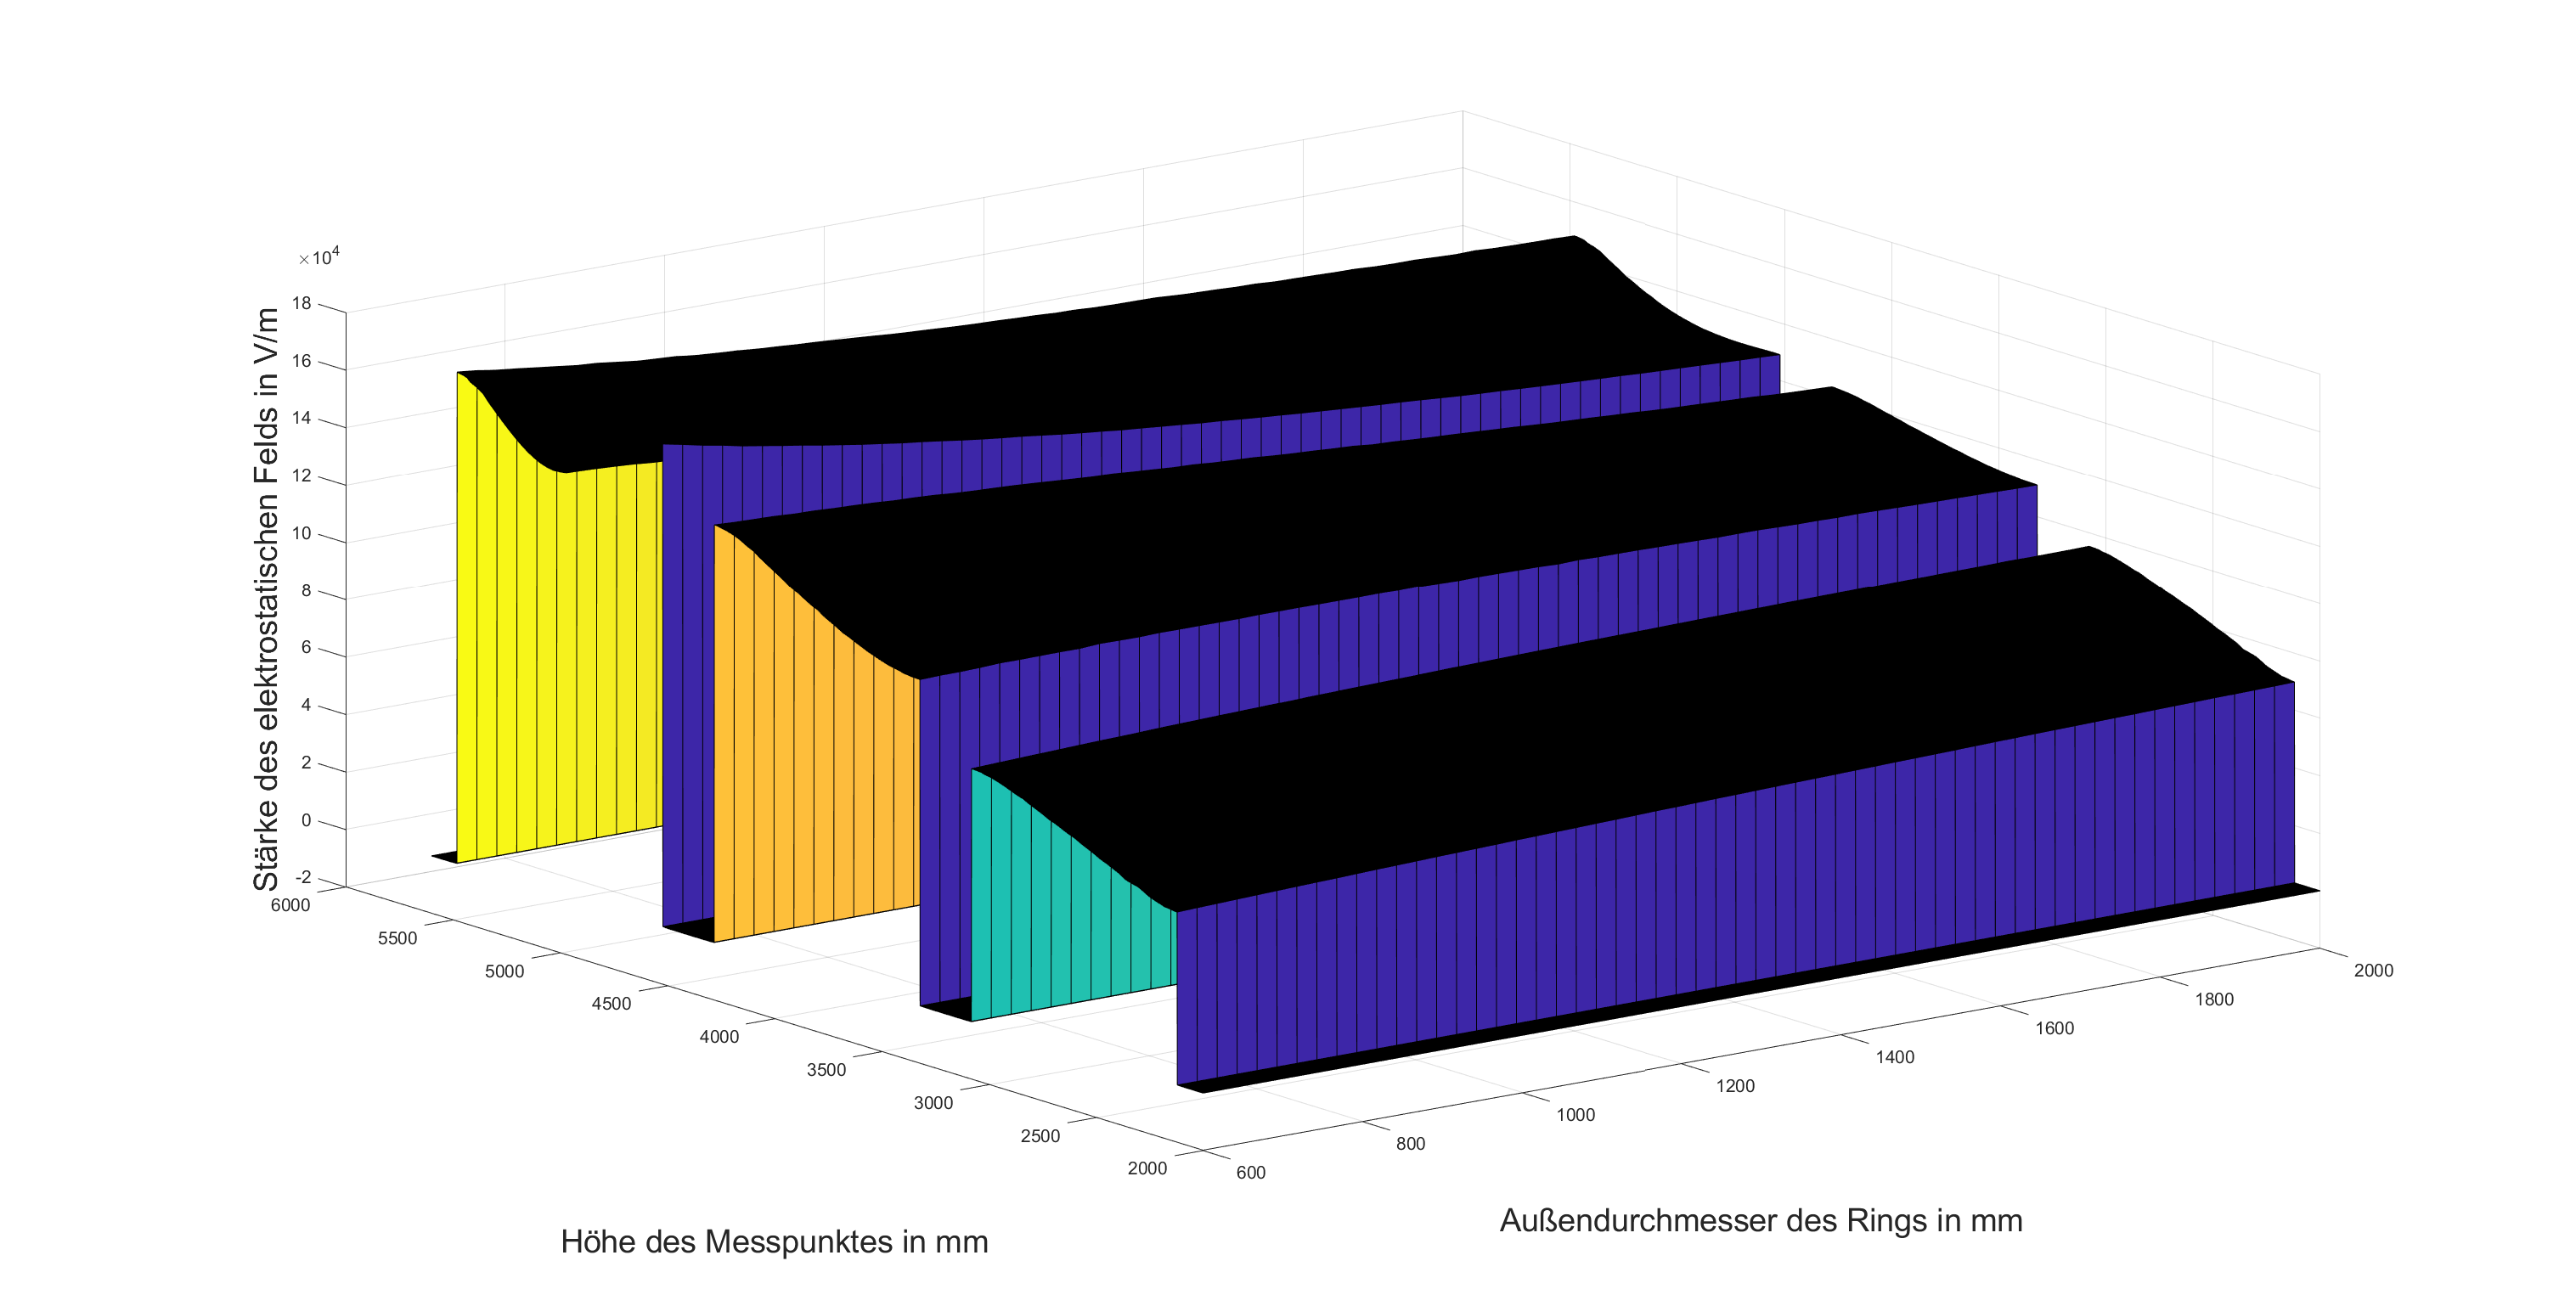
\includegraphics[width=\textwidth]{data/3DEtang}
	\end{subfigure}
	\begin{subfigure}[h]{\textwidth}
		\centering
		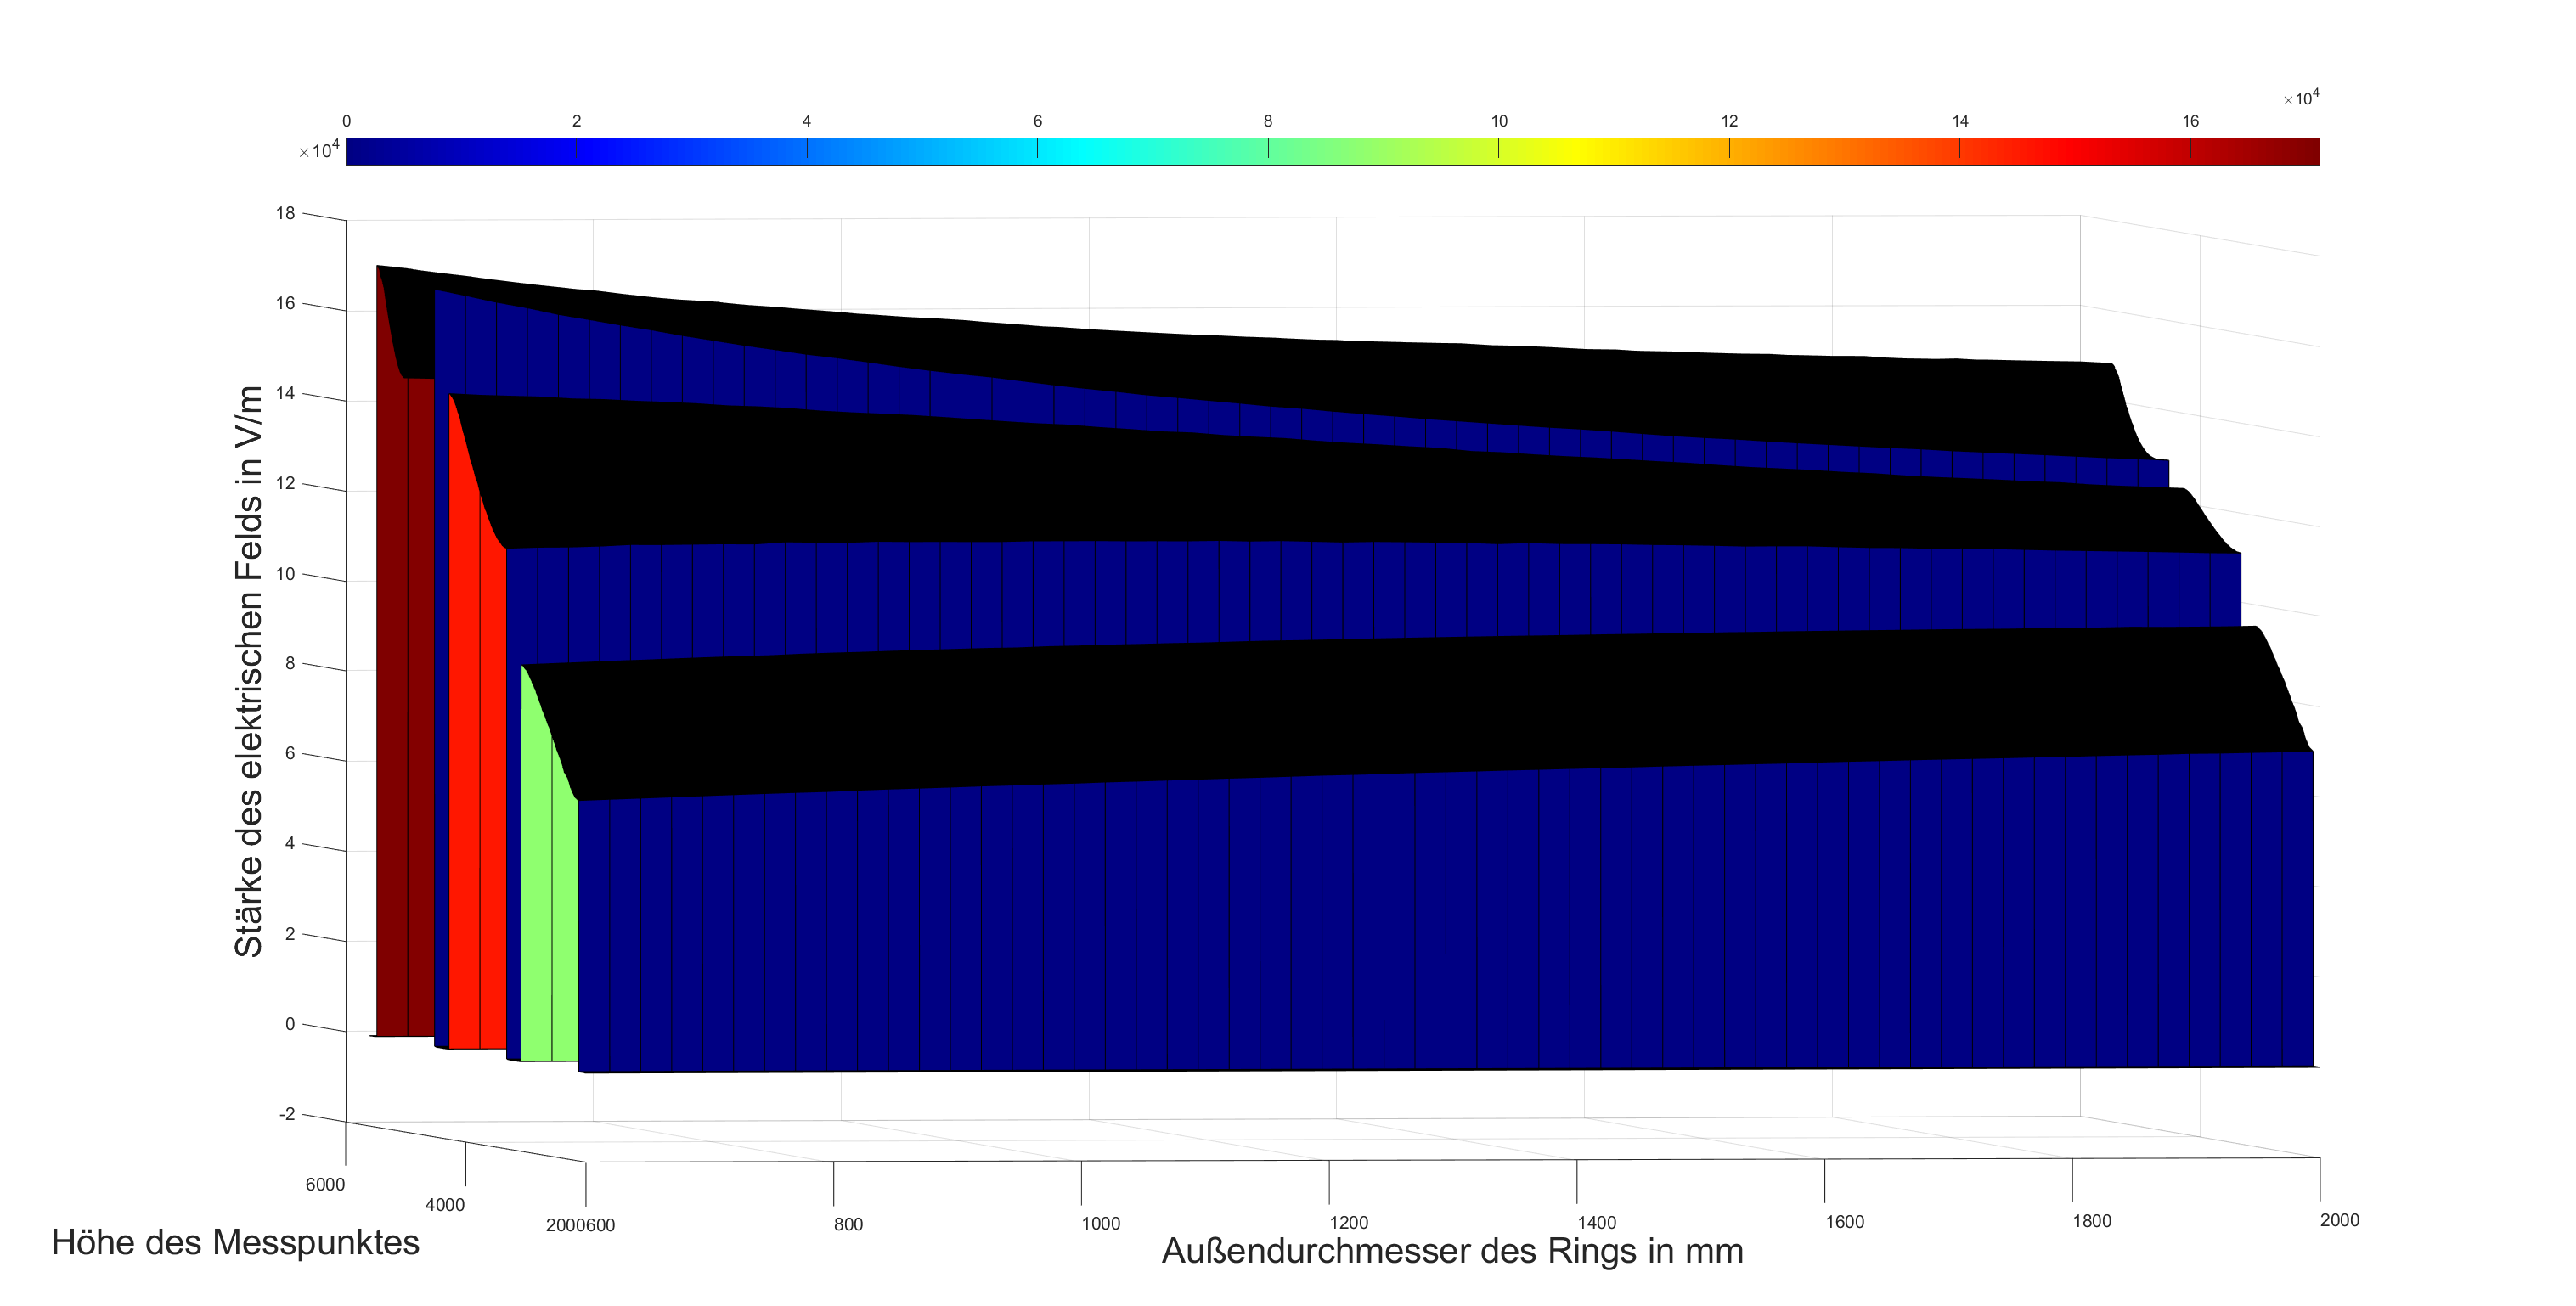
\includegraphics[width=\textwidth]{data/3DEtangVergleich}
	\end{subfigure}
\caption{Das tangentiale elektrische Feld in Abhängigkeit des Außendurchmesser des Rings und der Höhe des Messpunktes}
\label{fig:3DTang}
\end{figure}




	\section{Kanonische Indizierung, FIT}

Bei der kanonischen Nummerierung werden die Punkte $P(n)$ vom Ursprung ausgehend in $x$-Richtung bis zum Ende durchlaufen und aufsteigend durchnummeriert. Anschließend geht man einen Schritt in $y$-Richtung und läuft dann wieder alle Punkte in $x$-Richtung durch. Dieses Vorgehen wird solange wiederholt bis auch in $y$-Richtung das Ende des Gitters erreicht wurde. Danach macht man einen Schritt in $z$-Richtung und verfährt von dort ausgehend genauso wie zuvor schon. Damit wird erreicht das jeder Punkt im Gitter eine eigenen eindeutige Nummerierung erhält. Für die Nummerierung der Gitterkanten $L_w(n)$ ist der kleinste Punkt an dem die Kante liegt ausschlaggebend und $w$ bezeichnet die Raumrichtung in der Kante, also $x$, $y$, oder $z$.
In Abbildung \ref{fig:primal} ist diese Art der Nummerierung graphisch dargestellt wobei die Knoten in blau beschriftet sind und die Kanten in grün.
\begin{figure}[h]
	\centering
	\includegraphics[width=\textwidth]{data/PrimalAllVertexAllEdge}
	\caption{Primales Gitter mit Beschrifteten Ecken und Kanten}
	\label{fig:primal}
\end{figure}

Dasselbe Vorgehen wie bei der primalen Gitterstruktur gilt nun auch für die dualen Objekte wie in Abbildung \ref{fig:dual} zu sehen ist. Dabei fällt auf dass die Nummerierung der Knoten des Dualen Gitters mit der Nummerierung der Volumen des Primalen Gitters übereinstimmen. Der Duale Knoten $\tilde{P}_1$ liegt also im Primalen Volumen $V_1$. Außerdem schneidet jede Kante des einen Gitters genau eine Fläche des anderen Gitters und auch jede Duale Zelle enthält genau einen primären Punkt. Auf diese Art zusammengehörende Objekte haben immer die gleiche Indizierung.
 
\begin{figure}[h]
	\centering
	\includegraphics[width=\textwidth]{data/VolumenDualVertex}
	\caption{Primales Gitter(weiß) mit beschriftetem Dualem Gitter (orange)}
	\label{fig:dual}
\end{figure}
            	

	%%%%%%%%%%%%%%%%%%Fazit%%%%%%%%%%%%%%%%%%%%%%
	\chapter{Fazit}\label{sec:fazit}
%\addcontentsline{toc}{section}{Fazit}
Die erste Aufgabe ergab, dass sich die beiden Leiter des Koaxialkabels wie die Platten eines Plattenkondensators verhalten. Darüber hinaus ergibt sich, dass man durch Anfügen von weiteren Segmenten an die Schaltung eine Verkleinerung der Schwingfrequenz bewirkt.
Differentialgleichungen können häufig, wie sich in Aufgabe zwei zeigt, leichter im Frequenzbereich als im Zeitbereich gelöst werden. Die durch Lösen der Differentialgleichung analytisch berechneten Ergebnisse für Zeit- und Frequenzverhalten stimmen dabei mit der numerischen Simulation durch LTSpice überein.
Die Ergebnisse der dritten Aufgabe ergeben, dass sich die Feldlinien eines Kondensators in einem Simulationskäfig nicht nur senkrecht zu den Platten bewegen, sondern dass sich auch Randeffekte an den Enden der Kondensatorplatten ausbilden. Untersucht man unterschiedliche Randbedingungen zeigt sich, dass diese sowohl den Kapazitätswert des Kondensators, als auch die elektrischen Feldlinien beeinträchtigen. Die Wahl der Simulationsrandbedingungen kann also nicht willkürlich erfolgen.
	%%%%%%%%%%%%%%%%%%Anhang%%%%%%%%%%%%%%%%%%%%%
	\chapter{Anhang}\label{sec:anhang}
%\addcontentsline{toc}{section}{Anhang}
Dies ist der Anhang.
	%%%%%%%%%%%%%%%%%%%%%%%%%%%%%%%%%%%%%%%%%%%%%%%%%%%%%%%%%%%%%%%%%%%%%%%%%%%%%%%%%%%%%%%%%%%%%%%%%%
	
	%%%%%%%%%%%%%%%%%%%
	%Abbildungs- und Tabellenverzeichnis
	%%%%%%%%%%%%%%%%%%%
	\listoffigures % Abbildungsverzeichnis (captions in den Figuren werden als Referenz genommen)
	%\listoftables % Verzeichnis der Tabellen (captions in den Tabellen werden als Referenz genommen)
	
	%%%%%%%%%%%%%%%%%%%
	%Literaturverzeichnis an dieser Stelle
	%%%%%%%%%%%%%%%%%%%
	
	
\end{document}
